\documentclass[paper=a4, fontsize=11pt]{scrartcl}
\usepackage[T1]{fontenc}
\usepackage{fourier}

\usepackage[english]{babel}
\usepackage[protrusion=true,expansion=true]{microtype} 
\usepackage{amsmath,amsfonts,amsthm,amssymb}
\usepackage[pdftex]{graphicx} 
\usepackage{url}

\usepackage{float}

\usepackage{tikz} 
\usepackage{tikzscale}

\usepackage{parskip}

\usepackage{hyperref}
\hypersetup{colorlinks=true, citecolor=black, linkcolor=black, urlcolor=blue}
\urlstyle{same}

\usepackage{subfigure}

\usepackage{caption}

\usepackage[outputdir=out]{minted}
\usemintedstyle{tango}
\setmintedinline{breaklines}

\newtheorem{proposition}{Proposition}

\usepackage{sectsty}
\allsectionsfont{\centering \normalfont\scshape}
\usepackage{fancyhdr}
\pagestyle{fancyplain}
\fancyhead{}
\fancyfoot[L]{}
\fancyfoot[C]{}
\fancyfoot[R]{\thepage}
\renewcommand{\headrulewidth}{0pt}
\renewcommand{\footrulewidth}{0pt}
\setlength{\headheight}{13.6pt}

\newcommand{\horrule}[1]{\rule{\linewidth}{#1}}

\title{
    \usefont{OT1}{bch}{b}{n}
    \normalfont \normalsize \textsc{Università degli Studi di Verona} \\ [15pt]
    Master's degree in computer science and engineering / Big Data \\ [15pt]
    \horrule{0.5pt} \\[0.4cm]
    \huge Counting the number of triangles in a very large graph using the TTP algorithm \\
    \horrule{2pt} \\[0.5cm]
}
\author{
    \normalfont \normalsize
    Elia Perantoni, VR472361
    \\[-3pt] \normalsize \today
}
\date{}

\begin{document}
\maketitle
\section{Introduction}
A triangle $\Delta(u, v, x)$ in a undirected graph $G=(V, E)$ is a triple of
nodes $u, v, x$ such that all edges between them are in $E$. That is: $\{(u,v),
(u,x), (v, x)\}\subseteq E$.

\begin{figure}[htb]
    \centering
    \begin{tikzpicture}[node distance={15mm}, thick, every node/.style={draw, circle, minimum size=22pt}]
        \node (u) {$u$}; 
        \node (v) [below left of=u] {$v$}; 
        \node (x) [below right of=u] {$x$};
        \draw (u) -- (v) -- (x) -- (u);
        \node (a) [left of=v] {$a$};
        \node (b) [below left of=a] {$b$};
        \node (c) [below right of=x] {$c$};
        \draw (v) -- (a) -- (b);
        \draw (x) -- (c);
    \end{tikzpicture}
    \caption{A triangle $\Delta(u, v, x)$ inside a larger graph}
\end{figure}

The problem of counting triangles in a graph inherits great importance from
several interesting metrics on graphs that build upon it. The clustering
coefficient, for instance, is a measure of the degree to which nodes in a graph
tend to cluster together. Evidence suggests that real world graphs, social
networks in particular, tend to create tightly knit groups characterized by a
relatively high density of ties. This metric, arguably a very insightful one,
requires the number of triangles to be known, in order to compute it. Hence, its
relevance.

In recent years, internal and external memory algorithms have been developed to
solve the problem of triangle counting; but some of the graphs that we wish to
analyze have become so large that they can no longer fit inside a single
machine.

A popular technique for distributed computation is \emph{Map-Reduce}: a
\emph{map} function is applied to each element in the input collection
individually to produce key-value pairs, the shuffle phase then merges all
values belonging to the same key and, finally, a \emph{reduce} function is
applied to each group of values (one for each key) to produce the final result.
What makes Map-Reduce so powerful is the fact that data can be split in
partitions to which the map and reduce functions can be applied independently.
With this mechanism, processing enormous quantities of data becomes possible as
the work can be distributed among a large number of machines.

This report comes with, and provides context to, a Jupyter notebook in which a
recently developed Map-Reduce algorithm known as \emph{TTP (Triangle Type
Partition)} \cite{park2013efficient} is implemented, tested, analyzed and
compared with one of its predecessor: \emph{GP (Graph Partition)}
\cite{suri2011counting}.

We will first be introducing and discussing GP before moving to TTP because the
two algorithms have many concepts in common but GP is easier to understand.

\section{The tools}
Arguably, the most known Map-Reduce implementation is \emph{Apache Hadoop},
which also provides a distributed file system for data persistence: \emph{HDFS
(Hadoop Distributed File System)}. However, using Hadoop is somewhat tedious as
the provided functionality is limited to plain Map-Reduce only. Also, HDFS comes
with sup-optimal performance as secondary storage is used.

\emph{Apache Spark} is a software based on Hadoop that provides the framework
and unified set of APIs for performing a wide range of distributed computation
operations that go beyond just simple Map-Reduce. Spark also improves on HDFS by
using what's known as: \emph{RDD (Resilient Distributed Dataset)}. It's a
managed data structure that gets sharded and distributed (possibly with
replication) among the machines belonging to the same cluster. What's different
from HDFS is that RDDs' shards are stored in internal memory, thus noticeably
improving the performance of read/write operations.

Our implementation is Apache Spark based.

\section{Graph Partition algorithm}
In GP \cite{suri2011counting}, the input graph $G=(V, E)$ is split into $\rho$
partitions ($G_0, G_1, \dots, G_{\rho-1}$) using a partitioning function $P$
such that $\forall u \in V \ldotp P(u) \in [0, \rho-1]$. This gives
$V=\bigcup_{i=0}^{\rho-1} V_i$ and $\forall_{i\neq j} \ldotp V_i \cap V_j =
\emptyset$.

3 partitions $G_i$, $G_j$ and $G_k$ can be combined into one 3-partition
$G_{ijk}$ by taking the union of the nodes $V_{ijk} \triangleq V_i \cup V_j \cup
V_k$ and inducing the edges from the original $G$. See fig. \ref{some3parts} for
some examples.

\begin{figure}[h]
    \centering
    \begin{tikzpicture}[main/.style={draw, circle, minimum size=22pt, inner sep=0pt}]
        \node[main] (1) at (2, 7) {1};
        \node[main] (2) at (0, 6) {2};
        \node[main] (3) at (2, 5) {3};

        \node[main] (4) at (5, 7) {4};
        \node[main] (5) at (7, 6) {5};
        \node[main] (6) at (5, 5) {6};

        \node[main] (7) at (1, 2) {7};
        \node[main] (8) at (0, 0) {8};
        \node[main] (9) at (2, 1) {9};

        \node[main] (10) at (5, 1) {10};
        \node[main] (11) at (6, 2) {11};
        \node[main] (12) at (7, 0) {12};

        \draw (1) -- (2) -- (3) -- (1);
        \draw (4) -- (5) -- (6) -- (4);
        \draw (8) -- (7) -- (9);
        \draw (10) -- (12) -- (11);

        \draw (4) -- (3) -- (6);
        \draw (7) -- (10) -- (6) -- (7);
        \draw (3) -- (7);

        \draw[dashed] (-1, 3.5) -- (8, 3.5);
        \draw[dashed] (3.5, -1) -- (3.5, 8);

        \node at (-1.5,5.25) {Partition 0};
        \node at (8.5,5.25) {Partition 1};
        \node at (-1.5,1.75) {Partition 2};
        \node at (8.5,1.75) {Partition 3};
    \end{tikzpicture}
    \caption{A simple graph divided into 4 partitions}
    \label{graph}
\end{figure}

\begin{figure}[h]
    \centering
    \subfigure[$G_{012}$]{
        \includegraphics[width=0.3\linewidth]{tikz/threeparts1}
    }
    \hspace{40pt}
    \subfigure[$G_{123}$]{
        \includegraphics[width=0.3\linewidth]{tikz/threeparts2}
    }
    \caption{Some 3-partitions from the graph in fig. \ref{graph}}
    \label{some3parts}
\end{figure}

The algorithm finds the triangles in every 3-partition $G_{ijk}$ with $0 \le i <
j < k \le \rho - 1$ and assigns a weight to each. The sum of weights across all
partitions will give the correct number of triangles in $G$.

Some triangles are seen in more than one 3-partition. Take a triangle $\Delta(u,
v, x)$ entirely contained within partition $G_0=(V_0, E_0)$ for instance, it
will be observed repeatedly in any 3-partition $G_{0jk}$ with $j,k\neq 0$. The
purpose of the weight system then is to counteract this effect, ensuring that
the sum of all weights emitted for a triangle is always $1$. 

The weight to emit for a triangle solely depends on the number of partitions
that its nodes span:
\[
    w(\Delta(u,v,x)) = \begin{cases}
        \frac{1}{\binom{\rho-1}{2}} & P(u) = P(v) = P(x)  \\
        \frac{1}{\rho-2} & P(u) = P(v) \vee P(v) = P(x) \vee P(u) = P(x) \\
        1 & \text{otherwise}
    \end{cases}
\]

\begin{proposition}
    The sum of weights emitted by GP for any given triangle $\Delta(u, v, x)$ is $1$.
\end{proposition}
\begin{proof}
    Trivially, exactly one of these must be true:
    \begin{enumerate}
        \item $\Delta(u, v, x)$ is entirely contained within a single partition $G_A$
        \item $\Delta(u, v, x)$ is entirely contained within two partitions $G_A$ and $G_B$
        \item $\Delta(u, v, x)$ spans three partitions $G_A$, $G_B$ and $G_C$
        with each node belonging to a different one
    \end{enumerate}
    Therefore, we proceed with a proof by cases:
    \begin{enumerate}
        \item $\Delta(u, v, x)$ appears in any 3-partition $G_{ijk}$ where
        either $i$, $j$ or $k$ is equal to $A$. Therefore, two variables remain
        free and their values are chosen between $\rho-1$ possible partitions
        (all except A). Hence, $\Delta(u, v, x)$ appears in $\binom{\rho-1}{2}$
        partitions. For each of those a weight equal to
        $\frac{1}{\binom{\rho-1}{2}}$ is emitted, giving
        $\binom{\rho-1}{2}*\frac{1}{\binom{\rho-1}{2}}=1$.

        \item $\Delta(u, v, x)$ appears in any 3-partition $G_{ijk}$ with $\{i,
        j, k\} \subseteq \{A, B\}$. This means that one variable remains free
        and its value must be chosen among $\rho-2$ possible partitions (all
        except $A$ and $B$). Hence, $\Delta(u, v, x)$ appears in $\rho-2$
        partitions. For each of those a weight equal to $\frac{1}{\rho-2}$ is
        emitted, giving $(\rho-2)*\frac{1}{\rho-2}=1$.

        \item $\Delta(u, v, x)$ appears just in $G_{ABC}$. The weight $1$ will
        be emitted just once, trivially making the sum equal to $1$.
    \end{enumerate}
\end{proof}

The \emph{map} step consists of emitting an edge for every 3-partition that it
belongs to. The \emph{reduce} step is given a complete 3-partition and its job
is that of enumerating the triangles and emitting a weight for each. A
subsequent Map-Reduce pass is required to sum up the weights, giving the final
result.

The distributed nature of GP emerges when observing that the actual triangle
counting process can be performed on every 3-partition independently, using any
internal memory algorithm.

Depending on the size of $G$, a sufficiently large number of partitions $\rho$
will make sure that each is sufficiently small to fit inside a single machine.

The main issues with GP is that edges are emitted many times over, to account
for all 3-partitions in which they appear, and triangles are processed
redundantly. Take a triangle entirely contained within a single partition for
instance, with $\rho=10$. It will be processed in $\binom{\rho-1}{2}=36$
different 3-partitions. The improved algorithm, TTP, brings that number down to
just 9.

\section{Triangle Type Partition algorithm}

The TTP algorithm \cite{park2013efficient} improves on GP by reducing the amount
of redundancy and thus, the amount of data transferred in the cluster.

First, we formally classify triangles much in the same way as we did before for
our proof:
\begin{description}
    \item[Type I] Is a triangle $\Delta(u, v, x)$ spanning 1 partition
    \item[Type II] Is a triangle $\Delta(u, v, x)$ spanning 2 partitions
    \item[Type III] Is a triangle $\Delta(u, v, x)$ spanning 3 partitions
\end{description}

For instance, in fig. \ref{graph} $\Delta(1,2,3)$ is a Type I triangle,
$\Delta(3,4,6)$ is a Type II triangle and $\Delta(3,6,7)$ is a Type III
triangle.

Then, edges are also classified as being either \emph{inner} or \emph{outer}. An
edge $(u,v)$ is said to be inner when $u$ and $v$ belong to the same partition.
Otherwise, it's an outer edge.

A 3$^\prime$-partition (note the prime), denoted $G^{\prime}_{ijk}$, is a
3-partition composed only of outer edges. TTP reduces redundancy by searching
for Type III triangles in 3$^\prime$-partitions while and Type I and II
triangles in 2-partitions. In the future, we may refer to 2-partitions and
3$^\prime$-partitions as \emph{combinatorial partitions} to emphasize that they
are a combination of multiple $G_i$ ($i\in[0, \rho-1]$) partitions and to better
distinguish them.

See fig. \ref{ttp} for some examples of 2-partitions and 3$^\prime$-partitions.

\begin{figure}[h]
    \centering

    \subfigure[$G_{01}$]{
        \includegraphics[width=0.3\linewidth]{tikz/twoparts1.tikz}
    }
    \hspace{20pt}
    \subfigure[$G_{02}$]{
        \includegraphics[height=0.3\linewidth]{tikz/twoparts2.tikz}
    }
    \hspace{20pt}
    \subfigure[$G_{23}$]{
        \includegraphics[width=0.3\linewidth]{tikz/twoparts3.tikz}
    }

    \par\bigskip

    \subfigure[$G^\prime_{012}$]{
        \includegraphics[width=0.3\linewidth]{tikz/threepartsprime1}
    }
    \hspace{20pt}
    \subfigure[$G^\prime_{123}$]{
        \includegraphics[width=0.3\linewidth]{tikz/threepartsprime2}
    }
    \caption{Some examples of 2-partitions and 3$^\prime$-partitions from the
    graph in fig. \ref{graph}}
    \label{ttp}
\end{figure}

The interesting observation to make here is that Type III triangles are entirely
made up of outer edges and can therefore be correctly counted in
3$^\prime$-partitions that lack inner edges; thus making them smaller and
quicker to process. Additionally, Type I and Type II have at least one inner
edge, so they are not repeatedly processed in 3$^\prime$-partitions simply
because they don't exist there. The number of 3$^\prime$-partitions partitions
grows exponentially with $\rho$, so stripping them of inner edges and only
processing Type III triangles there makes for a big performance improvement.

The overall structure of the TTP algorithm is similar to that of GP: the
\emph{map} step emits a pair $(p, e)$ for every edge $e$ that belongs to
partition $p$, then the \emph{reduce} step receives an entire partition (that
might be a 2-partition or a 3$^\prime$-partition) and emits a weight for each
triangle found there. The sum of all weights emitted gives the total number of
triangles in the initial graph $G$.

In TTP, the weights are as follows:
\begin{equation} \label{ttpweights}
    w(\Delta(u,v,x)) = \begin{cases}
        \frac{1}{\rho-1} & P(u) = P(v) = P(x)  \\
        1 & \text{otherwise}
    \end{cases}
\end{equation}
So Type I triangles get $\frac{1}{\rho-1}$ while Type II and Type III triangles
get $1$.

\begin{proposition}
    The sum of weights emitted by TTP for any given triangle $\Delta(u, v, x)$ is $1$.
\end{proposition}
\begin{proof}
    Every triangle is either Type I, Type II or Type III. Let's proceed with a
    proof by cases.
    \begin{description}
        \item[Type I] Suppose $\Delta(u, v, x)$ is entirely contained within
        partition $G_A$. Then, it appears in all 2-partitions $G_{ij}$ with
        $i=A$ or $j=A$. It cannot appear in 3$^\prime$-partitions because a Type
        I triangle is entirely made out of inner edges, which
        3$^\prime$-partitions lack. Therefore, there are $\rho-1$ partitions in
        which the triangle appears. And every time that happens a weight equal
        to $\frac{1}{\rho-1}$ is emitted. Giving $(\rho-1)*\frac{1}{\rho-1}=1$.

        \item[Type II] Suppose $\Delta(u, v, x)$ is entirely contained within
        partition $G_A$ and $G_B$ (suppose also wlog that $A<B$). Then, it
        appears only in 2-partition $G_{AB}$. It cannot appear in
        3$^\prime$-partitions because a Type II triangle has one inner edge,
        which 3$^\prime$-partitions lack. Therefore, there is just one partition
        in which the triangle appears. Since $1$ is emitted just once, the sum
        is trivially equal to $1$.

        \item[Type III] Suppose $\Delta(u, v, x)$ spans three partitions $G_A$,
        $G_B$ and $G_C$ (suppose also wlog that $A<B<C$). Then, it appears only
        in 3$^\prime$-partition $G_{ABC}$. It cannot appear in 2-partitions
        simply because the triangle is composed of nodes from three distinct
        partitions. Since $1$ is emitted just once, the sum is trivially equal
        to $1$.
    \end{description}
\end{proof}

\section{Datasets} \label{datasets}
For this project, undirected graphs from the
\href{http://snap.stanford.edu/data/index.html}{Standford Large Network Dataset
Collection} were used. In particular, the software is tested against these (in
order of disk size):
\begin{enumerate}
    \item ego-Facebook (1612010 triangles)
    \item email-Enron (727044 triangles)
    \item com-Amazon (667129 triangles)
    \item roadNet-CA (120676 triangles)
\end{enumerate}

To make the whole algorithm easier to understand and reason about, the same
example from \cite{park2013efficient} is also used before getting to more
complicated datasets.

Each dataset is given as a text file in the \mintinline{text}{datasets/}
directory. Nodes are identified by means of a unique integer and for each edge
$(u,v) \in E$ there is a line in the file with the node ids of $u$ and $v$,
separated by whitespace. \emph{Edges are not reported twice}, meaning there is
no \mintinline{text}{"v u"} line when \mintinline{text}{"u v"} is already there.

\section{Implementation in depth}
In this section, we are going to walk through the implementation provided along
with this report as a Jupyter notebook. The same example graph used in
\cite{park2013efficient} (also shown in fig. \ref{graph}) will be used
throughout.

First, we load the dataset from disk and perform some preprocessing to make
everything easier.
\begin{minted}{python}
edges = (sc
    .textFile(DATASET)
    .filter(bool)                     # Discard empty lines
    .map(lambda line: line.split())   # Split nodes in edge
    .map(lambda x: list(map(int, x))) # Parse node ids
    .map(tuple))                      # Convert list to tuple
\end{minted}
The call to \mintinline{python}{textFile} returns an RDD whose elements are
lines from the dataset's file. We filter out empty lines using the
\mintinline{python}{bool} built-in function, then split each line by whitespace
to get a pair of node ids, both of which are parsed to integers. Then the pair
of nodes, thus far represented with a list of length 2, is converted to a tuple,
just for personal preference.

If we were to collect \mintinline{python}{edges}, the result would look
something like: \mintinline{python}{[(1, 2), (1, 3), (2, 3), (4, 5), (4, 6),
...]}. Each tuple in the list is a pair of node ids representing an undirected
edge.

Next, we partition the graph by defining the number of partitions $\rho$ and a
partitioning function $P$. Note that the partitioning function initially used in
the notebook only works for the example graph shown in fig. \ref{graph} and was
chosen to mimic what's explained in \cite{park2013efficient}. A better, more
general, partitioning function will be provided later:
\begin{minted}{python}
RHO = 4
def P(node: int) -> int:
    return (node - 1) // (RHO - 1)
\end{minted}

Now we need to build the 2-partitions and 3$^\prime$-partitions that will be
distributed among workers for independent triangle counting. This process works
by producing a set $\{(p,e)\}$, where each element $(p,e)$ is stating that edge
$e$ belongs to the combinatorial $p$, and grouping by $p$ to obtain all the
edges for that partition.

\mintinline{python}{edges_in_2p_map} and \mintinline{python}{edges_in_3p_map}
are the mapping functions that take an edge $e\in E$ and map it to all $(p,e)$
such that $p$ is a 2-partition or a 3$^\prime$-partition respectively, and $e$
belongs to $p$:
\begin{minted}{python}
def edges_in_2p_map(edge):
    u, v = edge
    res = []
    for a in range(0, RHO - 1):
        for b in range(a + 1, RHO):
            if P(u) in [a, b] and P(v) in [a, b]:
                res.append(((a, b), (u, v)))     
    return res

def edges_in_3p_map(edge):
    u, v = edge
    if P(u) == P(v):
        return []
    res = []
    for a in range(0, RHO - 2):
        for b in range(a + 1, RHO - 1):
            for c in range(b + 1, RHO):
                if P(u) in [a, b, c] and P(v) in [a, b, c]:
                    res.append(((a, b, c), (u, v)))
    return res
\end{minted}
Notice that, because inner edges never appear in 3$^\prime$-partitions, if for
an edge $e=(u,v)$ we have $P(u)=P(v)$ then \mintinline{python}{edges_in_3p_map}
completely skips it.

We map all the edges in the graph using both functions in parallel and flatten
the results. The flattening step is necessary because each edge produces not
just one $(p,e)$ pair but many of them instead.

We end up with two sets $\{(p,e)\}$: the first only contains pairs
$(p,e)$ where $p$ is a 2-partition while the second only contains pairs $(p,e)$
where $p$ is a 3$^\prime$-partition. We take the union of those two sets:
\begin{minted}{python}
edges_in_2p = edges.flatMap(edges_in_2p_map)
edges_in_3p = edges.flatMap(edges_in_3p_map)
edges_in_Xp = edges_in_2p.union(edges_in_3p)
\end{minted}

If we now were to inspect \mintinline{python}{edges_in_Xp} we would see something
like:
\begin{minted}{python}
[((0, 1), (1, 2)),
 ((0, 2), (1, 2)),
 ((0, 3), (1, 2)),
 ((0, 1), (1, 3)),
 ((0, 2), (1, 3)),
 ...,
 ((0, 1, 2), (3, 6))
 ...,
]
\end{minted}
Meaning that edge $(1,2)$ belongs to partitions $G_{01}$, $G_{02}$ and $G_{03}$;
edge $(1,3)$ belongs to partitions $G_{01}$, $G_{02}$, etc... But also, maybe
more interestingly, edge $(3,6)$ belongs to partition $G^\prime_{012}$.

Noticing that we now have a collection of pairs where the partition occupies the
first position, we can \mintinline{python}{groupByKey} to collect all the edges
belonging to the same partition:
\begin{minted}{python}
# Merge together all the edges belonging to the same partition
edges_in_Xp_merged = edges_in_Xp.groupByKey()
\end{minted}

Now we are finally ready to count the triangles in every partition, emitting a
weight for each, and summing the results.

First, \mintinline{python}{assign_weight} is the function that takes a triangle
and assigns a weight to it. It's exactly an implementation of eq.
\ref{ttpweights}:
\begin{minted}{python}
# Will be used later on to avoid floating point arithmetic errors.
from fractions import Fraction

def assign_weight(triangle):
    u, v, x = triangle
    if P(u) == P(v) == P(x):
        # If triangle is Type I, then the weight is 1/(RHO-1).
        return Fraction(1, RHO-1)
    else:
        # For all other triangles, 1 because they are observed only once.
        return Fraction(1, 1)
\end{minted}

The usage of \mintinline{python}{Fraction}, instead of simply
\mintinline{python}{float}, is due to the fact that floating pointer numbers do
not have infinite precision and so slight errors can slowly creep up and lead to
wrong results. Here's a toy example to demonstrate the fact (Python 3.10.8):
\begin{minted}{python}
>>> 0.1 + 0.2
0.30000000000000004
\end{minted}

\mintinline{python}{Fraction} is a great alternative when one wishes to store
rational numbers with more precision because the numerator and denominator are
stored separately as integers:
\begin{minted}{python}
>>> Fraction(1, 10) + Fraction(2, 10)
Fraction(3, 10)
>>> float(Fraction(1, 10) + Fraction(2, 10))
0.3
\end{minted}

Now getting back to our algorithm, recall that we have a collection of $(p,
\{e\})$ elements. That is: for every combinatorial partition $p$ we have a list
of edges that belong to it. Now that we have grouped all edges belonging to the
same $p$, we can actually strip that away because that's not needed for inducing
a graph and counting triangles on it. Then we're left with a collection of
edge-sets $\{e\}$, each of which can be processed independently by applying
\mintinline{python}{total_partition_weight} to it:
\begin{minted}{python}
weights = (edges_in_Xp_merged
    .map(lambda x: x[1])
    .map(total_partition_weight))
\end{minted}

The job of \mintinline{python}{total_partition_weight} is that of inducing the
subgraph of the combinatorial partition, using the provided edge-set, and
emitting a weight for each triangle found there. Since this is performed on a
single combinatorial partition, much smaller than the entire graph $G$, and on
different workers, an internal memory algorithm for triangle enumeration can be
used. 

\cite{park2013efficient} cites many different internal memory algorithms in its
"Related Works" section but it doesn't really matter which one is used. Since
\mintinline{python}{total_partition_weight} is given a list of edges, we found
the \emph{edge-iterator algorithm} a pretty natural choice. It works by
iterating through all edges and, for each $(u,v)\in E$, taking the intersection
of the adjacency list of $u$ and of $v$. For any node $x$ in the intersection, a
triangle $\Delta(u,v,x)$ is recorded. Notice that this algorithm observes each
triangle three times. Therefore, proper measures should be in place to take this
into account. We're simply relying on Python's sets to remove duplicate
triangles.

\begin{minted}{python}
def total_partition_weight(edges):
    # Given the list of edges, build an adjacency list.
    adj = dict()
    for edge in edges:
        u, v = edge
        adj[u] = adj.get(u, set()) | {v}
        adj[v] = adj.get(v, set()) | {u}
        
    # Collect here the set of edges found in this partition.
    # Use a set to avoid duplication.
    triangles = set()
    for edge in edges:
        u, v = edge
        # Take the intersection of the adjacency list of u and v.
        # For each node x, a triangle (u,v,x) exists.
        triangles |= {frozenset((u,v,x)) for x in adj[u] & adj[v]}
    
    # For each triangle found in this partition, compute its weight.
    _sum = Fraction(0, 1)
    for triangle in triangles:
        _sum += assign_weight(triangle)
        
    # And return the sum of the weights.
    return _sum
\end{minted}

We use the list of edges to build an adjacency list for every node, then we run
the actual edge-iterator algorithm recording every triangle without duplication,
and finally we compute the weight for each triangle found in this combinatorial
partition and emit the partial sum.

\mintinline{python}{triangles} is a set of triangles but every triangle is, in
turn, a set of nodes. This is because changing the order of nodes in a triangle
does not make it any different. But standard sets cannot be added to other sets
because they are not hashable; to overcome this problem
\mintinline{python}{frozenset} must be used.

All that's left to do now is add all the partial sums coming the various
partitions into one \mintinline{python}{Fraction} and converting that to an
integer:
\begin{minted}{python}
# Sum the weight from every partition
round(weights.sum())
\end{minted}
And sure enough, we get 5, which is what we expected for the graph in fig.
\ref{graph}.

As soon as we swap the simplified partitioning function $P$ with a more general
one such as this:
\begin{minted}{python}
def P(node: int) -> int:
    return node % RHO
\end{minted}
Then we can start testing the implementation on more and larger graphs. We
successfully conducted tests on all the datasets in sect. \ref{datasets} and you
can see the results in the attached notebook.

\section{Impact of $\rho$}
And now for some performance analysis: how does the number of partitions $\rho$
affect the execution time and amount of data exchanged between workers in TTP?
Given that the total number of combinatorial partitions is $\binom{\rho}{2} +
\binom{\rho}{3}$, a lower value of $\rho$ will result in significantly less
combinatorial partitions to process (see fig. \ref{rho_comb}). But each
combinatorial partition is now larger, potentially making it impossible for a
combinatorial partition to fit inside a single machine anymore.

\begin{figure}[htb]
    \centering
    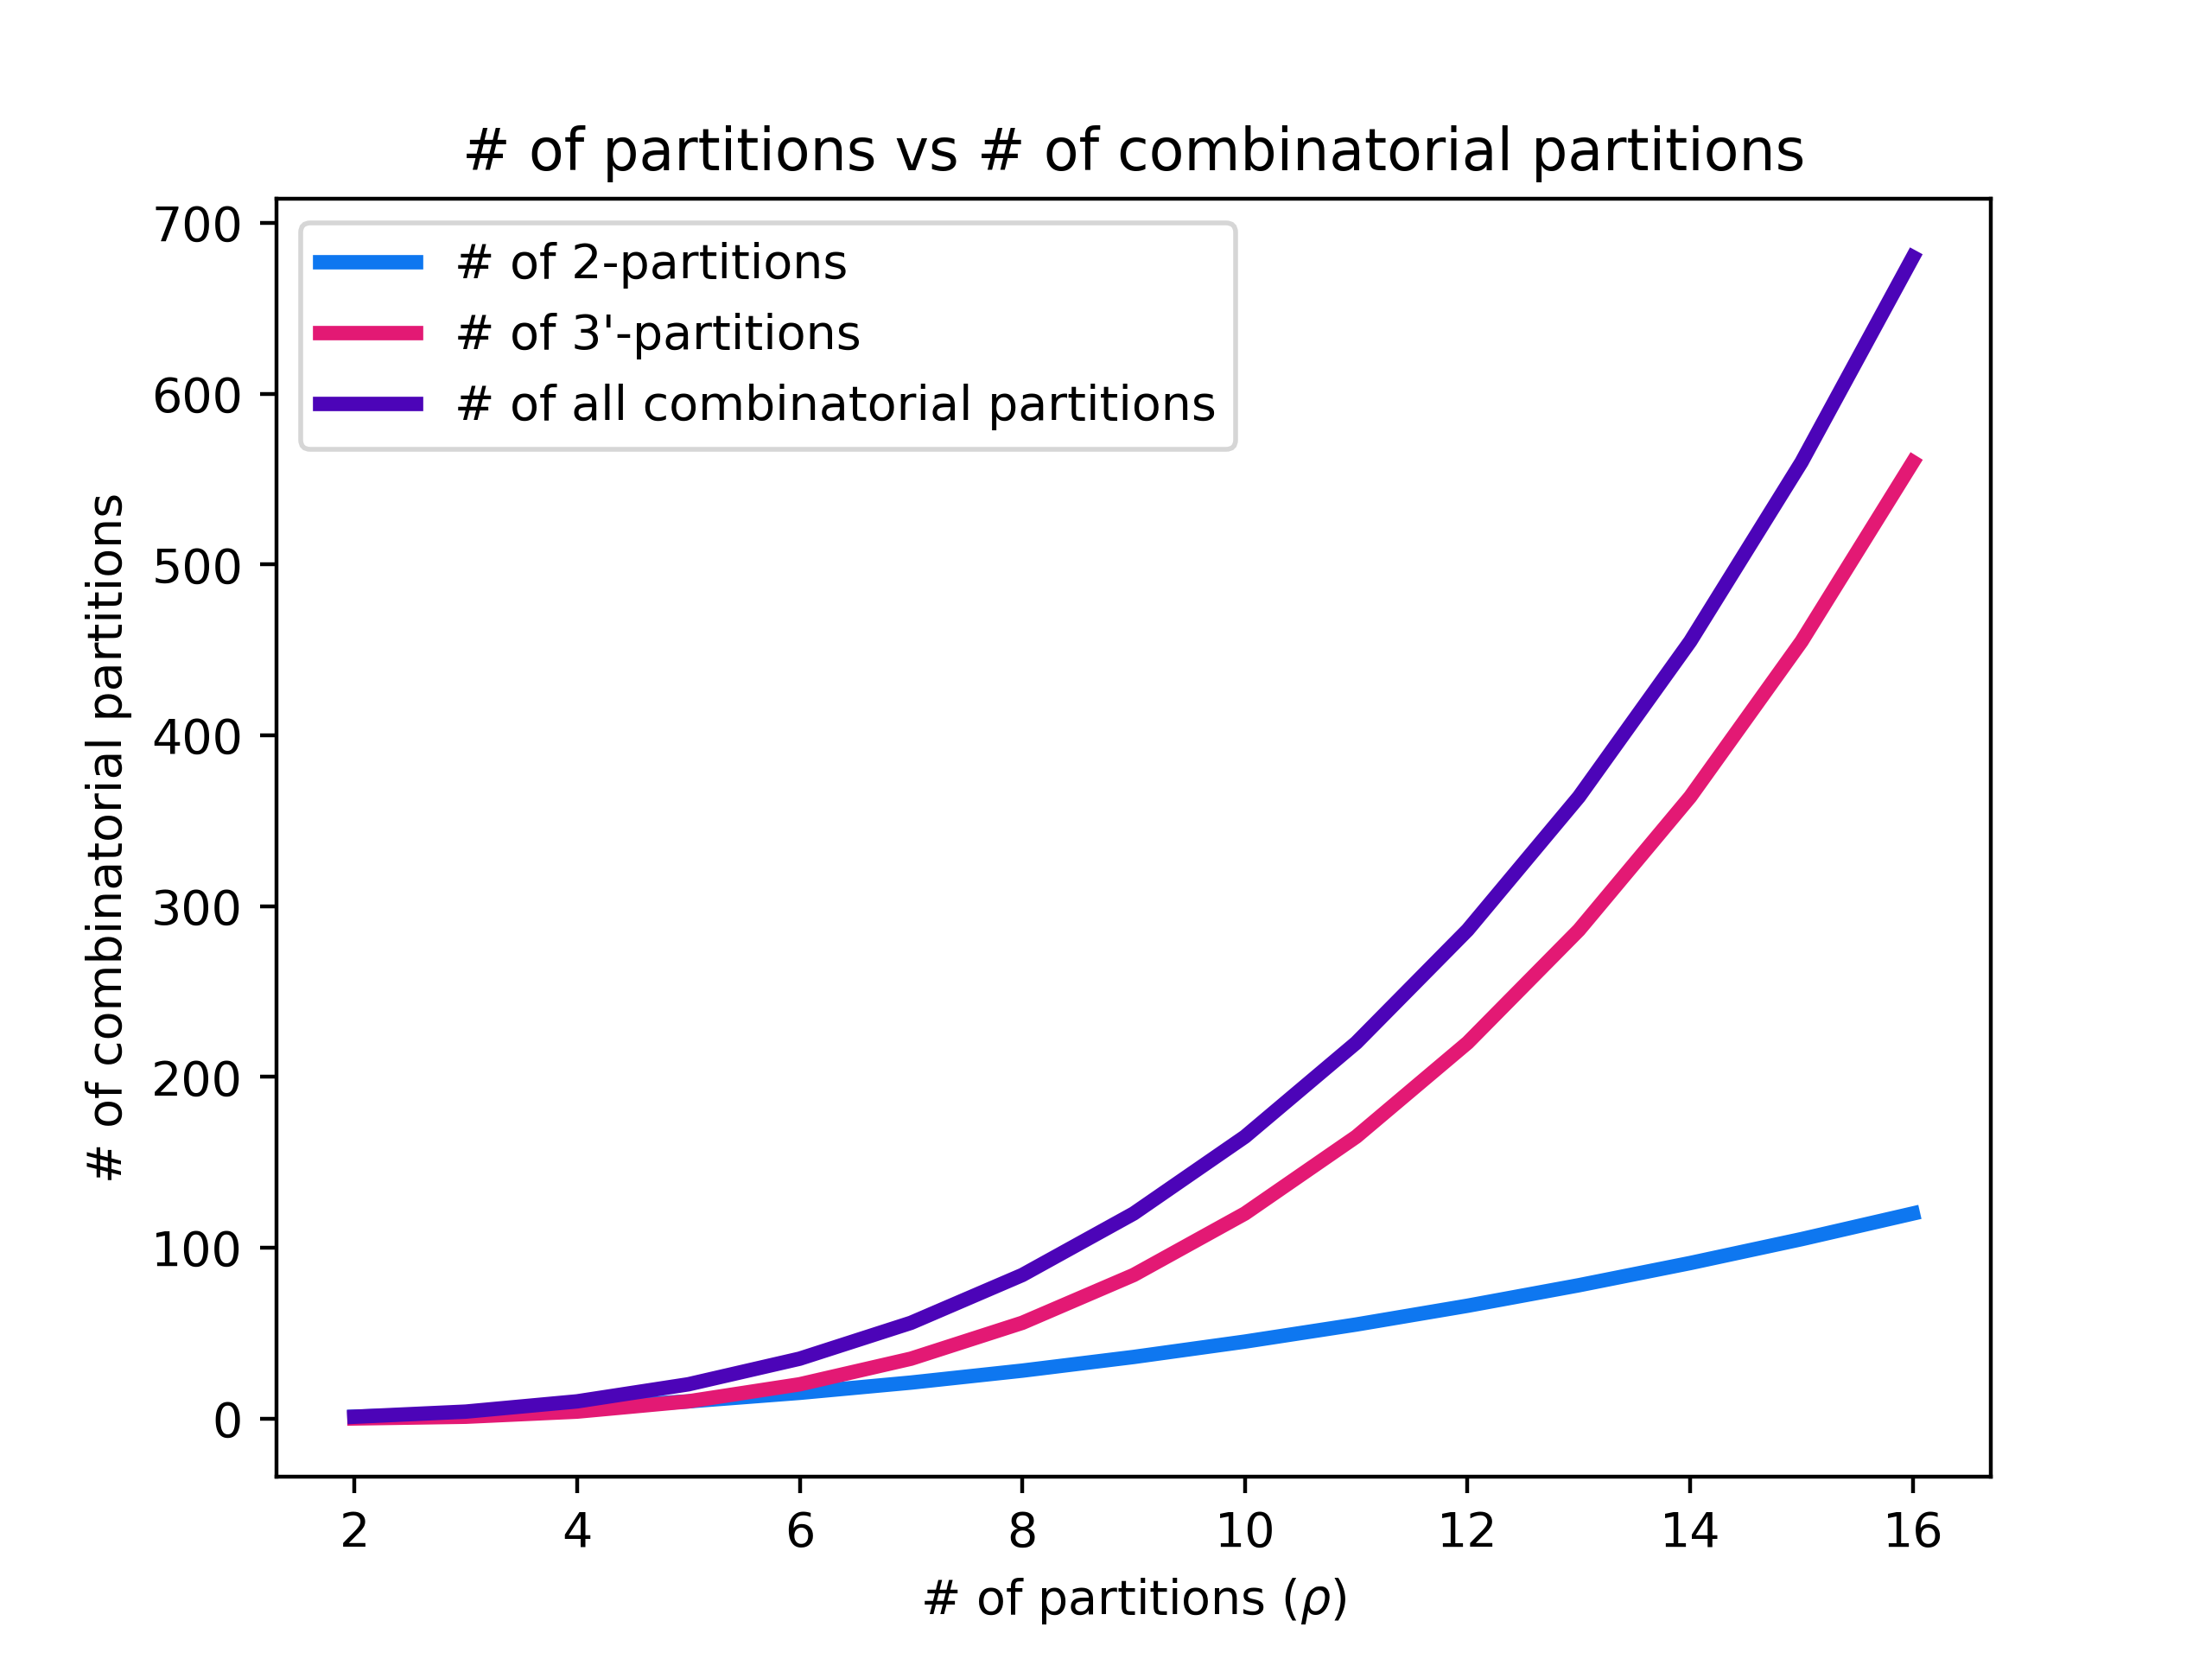
\includegraphics[width=0.7\textwidth]{img/rho_comb}
    \caption{} \label{rho_comb}
\end{figure}

Also, larger combinatorial partitions drive up the computational cost of the
internal memory algorithm used. This suggests that a tradeoff is at play and one
should not simply pick the lowest possible value of $\rho$ that allows all
combinatorial partitions to fit in the workers' memory.

To prove this point, we have benchmarked the algorithm with different values for
$\rho$ in $[2, 16]$ on the Ego Facebook datasets (see sect. \ref{datasets}). The
executions times are as observed by Python, since the Apache Spark admin console
is only precise down to the second.

\begin{figure}[htb]
    \centering
    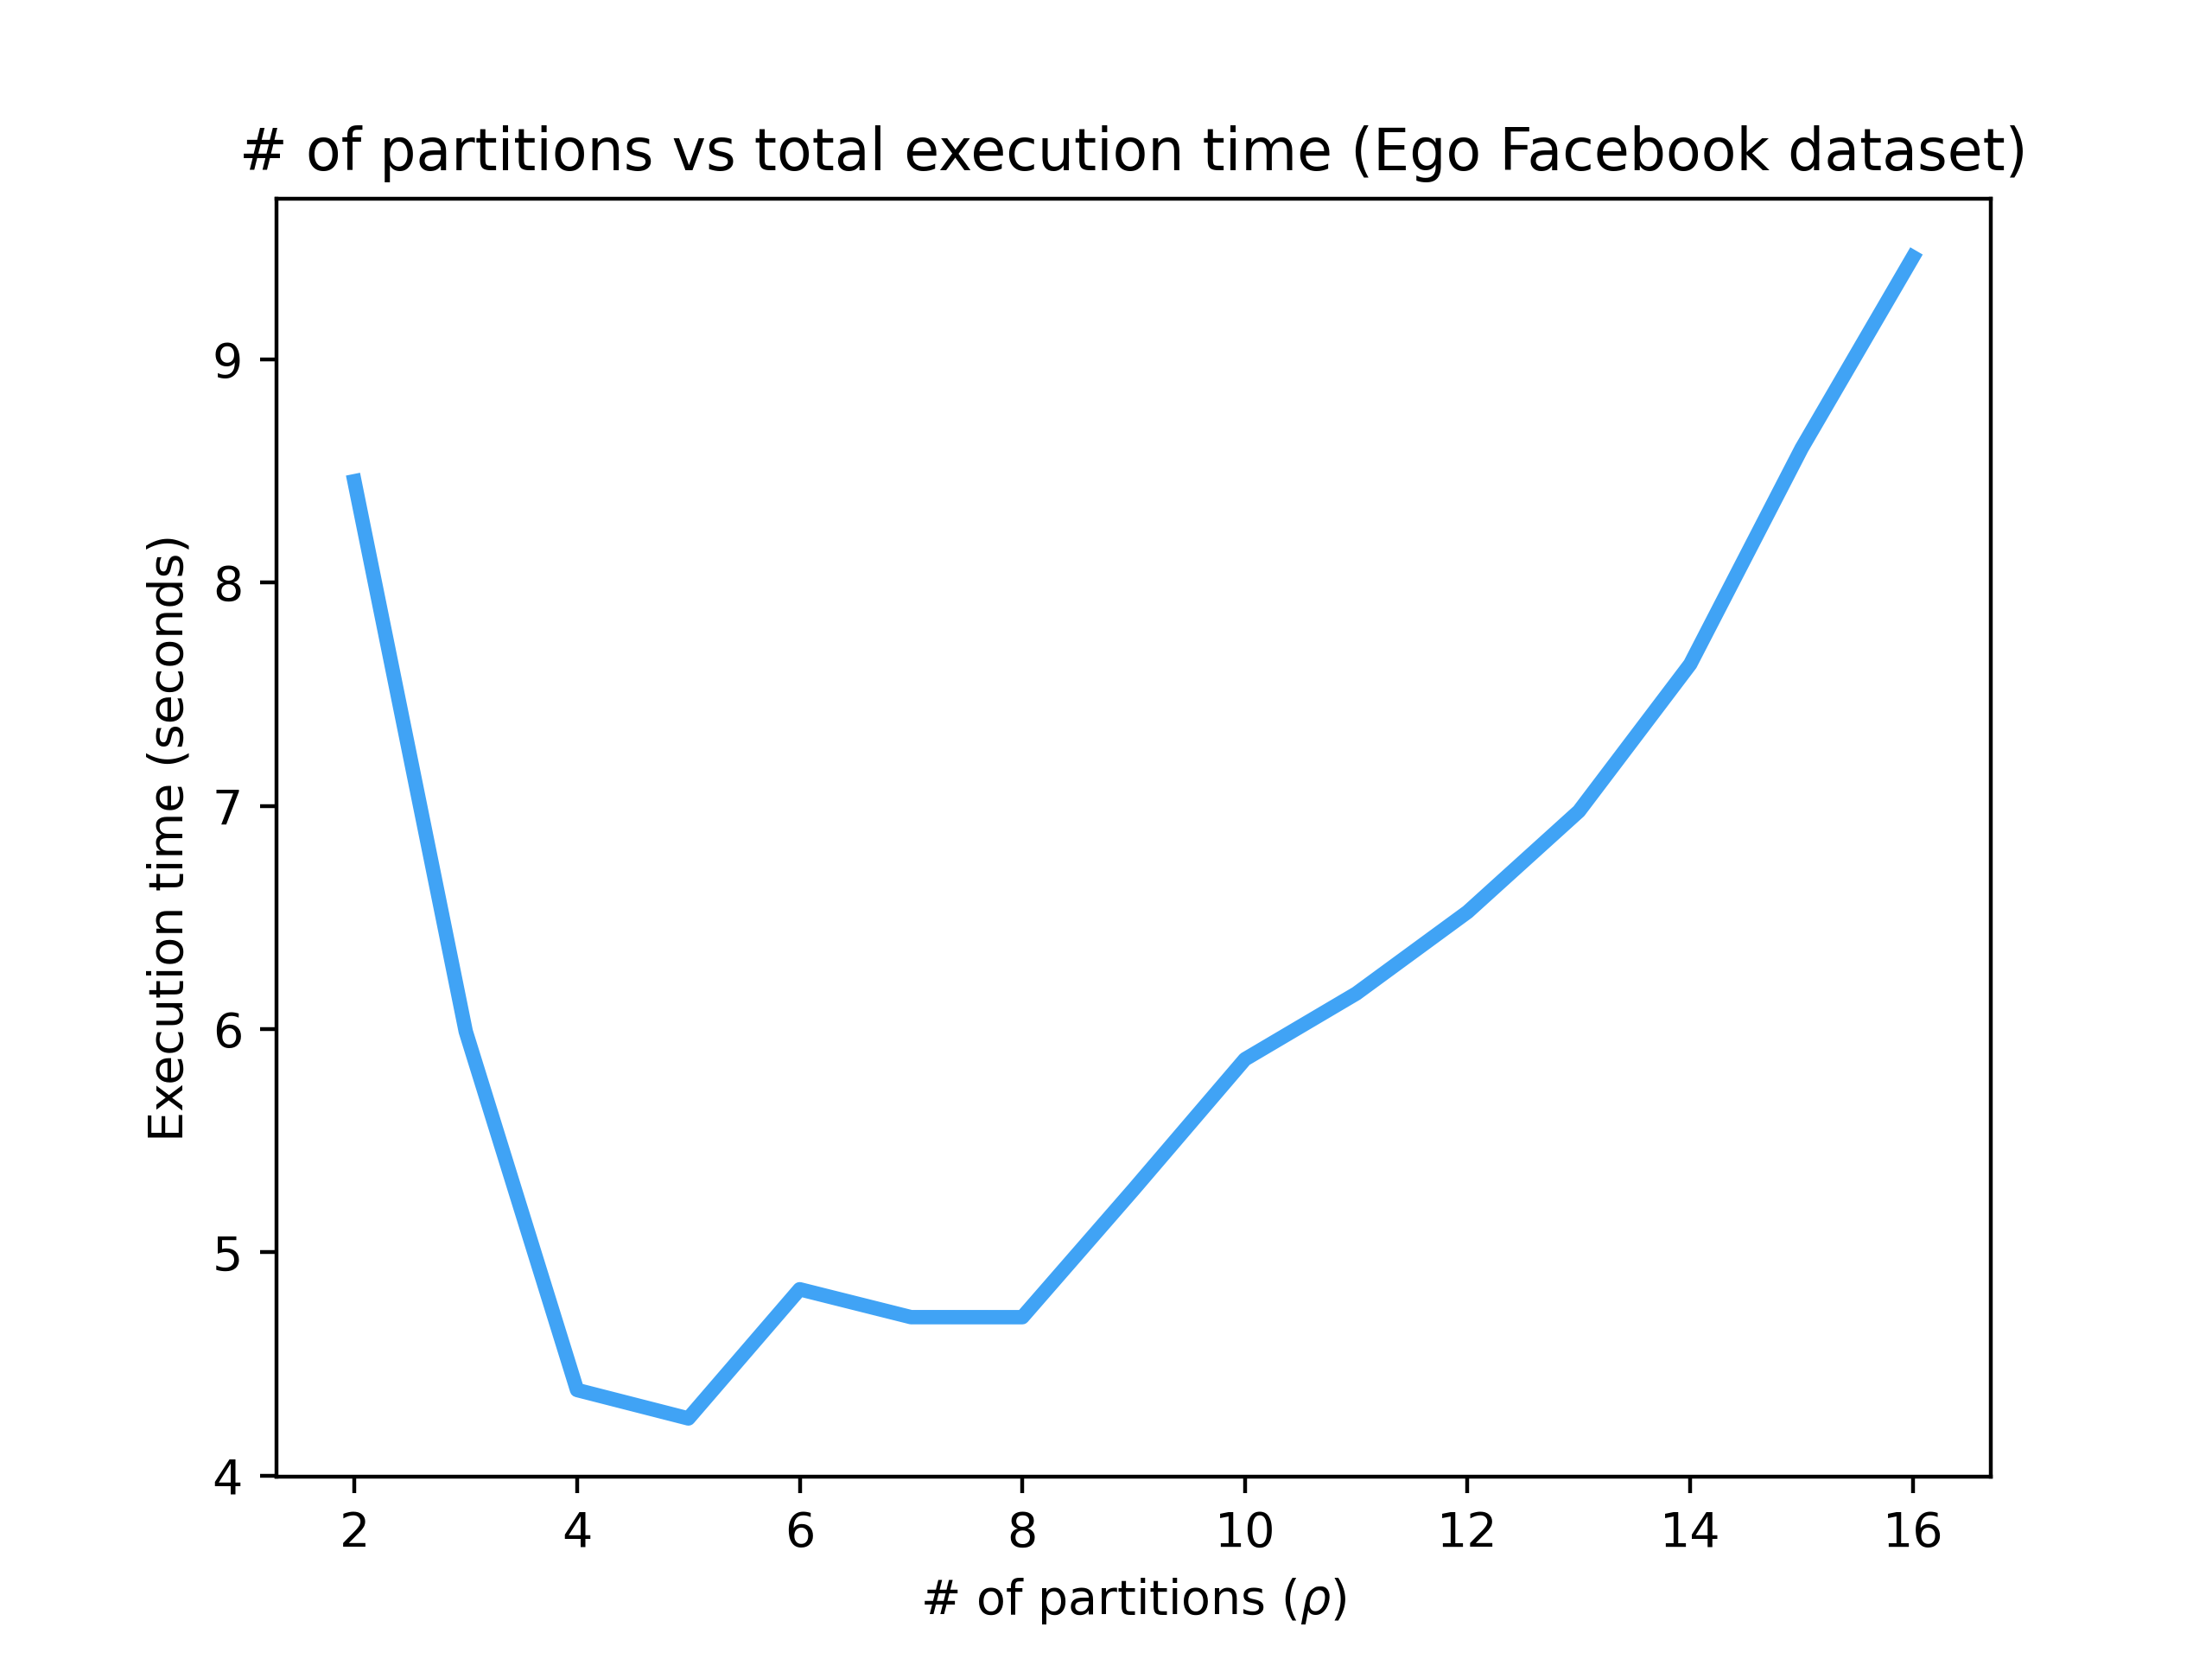
\includegraphics[width=0.7\textwidth]{img/rho_time}
    \caption{} \label{rho_time}
\end{figure}

On my machine, the best tradeoff seems to be around $\rho=4$ or $\rho=5$ (see
fig. \ref{rho_time}) but this is definitely dependent on the number of machines
in the cluster and their power. Point is: the lowest value for $\rho$ is not
necessarily the best.

Other factors that come into play are the amount of redundant processing of
triangles and the amount of Type I \& Type II triangles versus the amount of
Type III triangles. We've seen that as $\rho$ increases, the number of
combinatorial partitions increases. Therefore, a Type I triangle $\Delta(u,v,x)$
in partition $G_0$, for instance, is repeatedly counted in all 2-partitions
$G_{0j}$ with $j\in[1,\rho-1]$ and the number of those clearly increases with
$\rho$. On the other hand, a lower number of partitions means that more and more
triangles become Type I or Type II. The great thing about Type III triangles is
that they can be counted in stripped down subgraphs that are processed faster.
Having less of them is detrimental to the performance of the algorithm.

As you can tell, there is quite a large number of effects going in opposite
directions that depend on $\rho$, and predicting the best possible value is no
easy task.

If we shift our focus from execution time to amount of data exchanged during the
shuffle step, we see that it increases as $\rho$ increases, as one would expect
(fig. \ref{rho_data}).

\begin{figure}[htb]
    \centering
    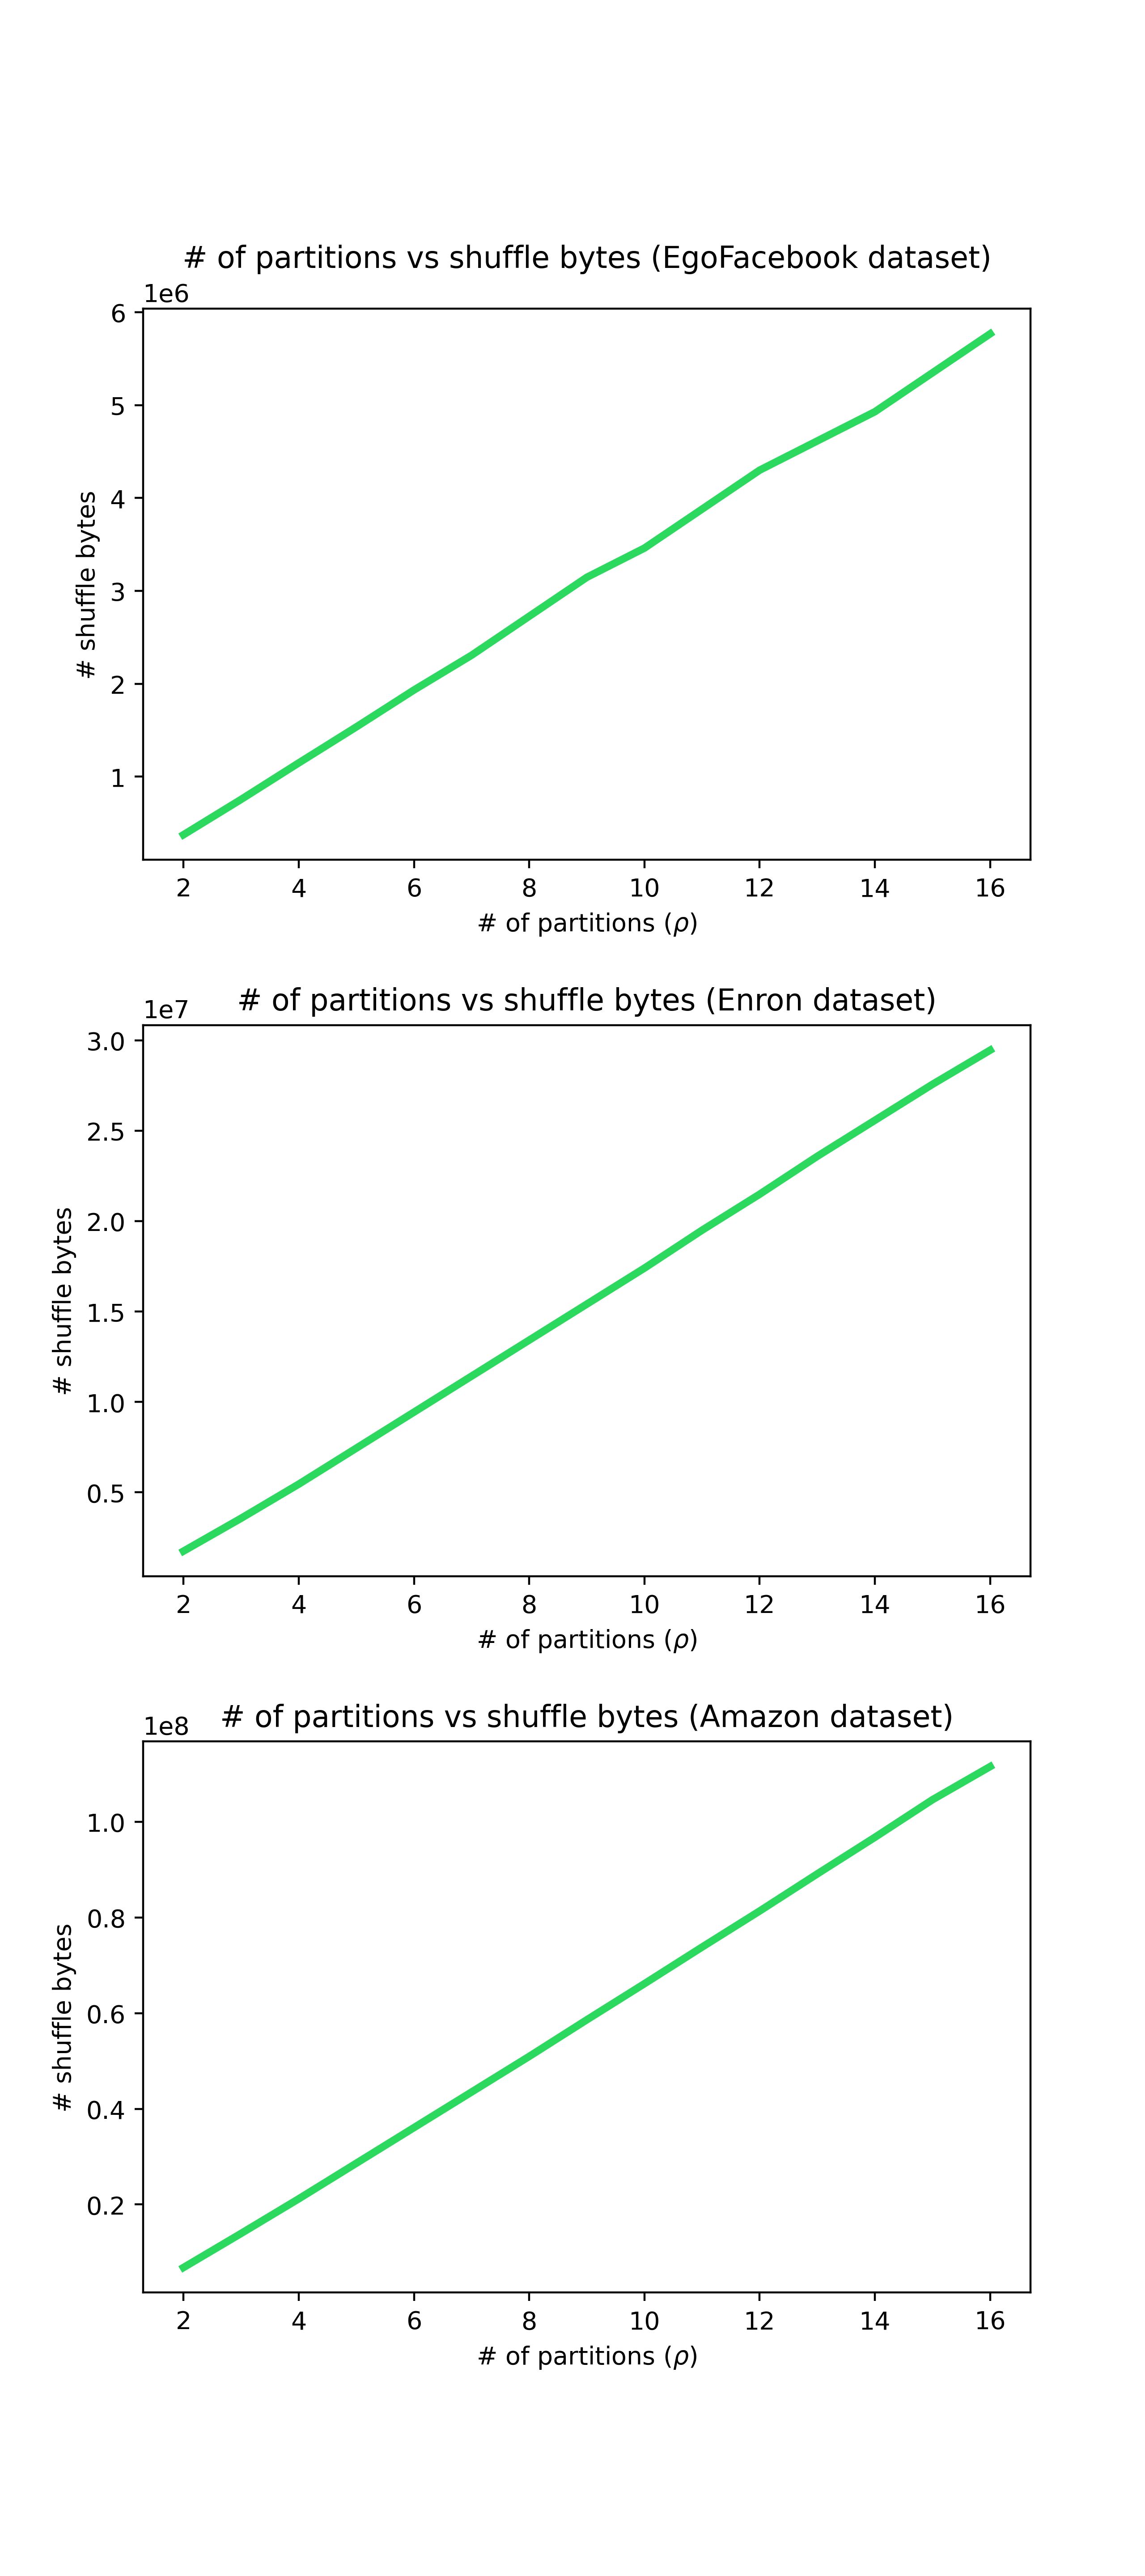
\includegraphics[width=0.7\textwidth]{img/rho_data}
    \caption{} \label{rho_data}
\end{figure}

(The amount of data was scraped from Spark's admin console using Python packages
\mintinline{text}{requests} and \mintinline{text}{beautifulsoup4}).

This can be explained by observing that a larger number of partitions $\rho$
makes for a larger number of combinatorial partitions, and this in turn results
in more duplication when emitting $(p,e)$ pairs: imagine an edge $(u,v)$
belonging to partition $G_0$, it is emitted in all $G_{0j}$ with $j\in[1,
\rho-1]$ and in all $G^\prime_{0jk}$ with $j,k\in[1, \rho-1]$. Obviously, with a
larger $\rho$ there are more $G_{0j}$ and $G^\prime_{0jk}$ for which to emit an
edge, driving up the amount of data exchanged.

\section{Performance comparison TTP vs GP}

\bibliographystyle{plain}
\bibliography{refs}
\end{document}
